\documentclass[conference]{IEEEtran}
\IEEEoverridecommandlockouts
% The preceding line is only needed to identify funding in the first footnote. If that is unneeded, please comment it out.
\usepackage{cite}
\usepackage{amsmath,amssymb,amsfonts}
\usepackage{systeme}
\usepackage{algorithmic}
\usepackage{graphicx}
\usepackage{textcomp}
\usepackage{xcolor}
\usepackage{flushend}
\usepackage{float}
\usepackage{lmodern}
\usepackage[]{algorithm2e}
\usepackage{times}
\usepackage[bookmarks=false]{hyperref}
\usepackage{pgfplots}
\usepackage{booktabs}
\usepackage{subfigure}
\usepackage[a4paper, left=0.51in, right=0.51in, top=0.75in, bottom=1.69in]{geometry}

\newcommand{\charly}[1]{{\color{red}[#1]}}		
\newcommand{\raffacel}[1]{{\color{blue}[#1]}}


\def\BibTeX{{\rm B\kern-.05em{\sc i\kern-.025em b}\kern-.08em
    T\kern-.1667em\lower.7ex\hbox{E}\kern-.125emX}}
    
    \IEEEoverridecommandlockouts
\IEEEpubid{%
\makebox[\columnwidth]{%
978-1-7281-7539-3/20/\$31.00~\copyright{}2020 IEEE\hfill%
} \hspace{\columnsep}\makebox[\columnwidth]{ }%
}
\begin{document}

\title{Análise de estudos de otimização de Algoritmos Genéticos (AG) por meio mutação e crossover dinâmicos}



\author{\IEEEauthorblockN{
        C. B. Ventura\IEEEauthorrefmark{1} and
        R. C. Carvalho\IEEEauthorrefmark{2}}
	\IEEEauthorblockA{\IEEEauthorrefmark{1,2}Institute of Technological Sciences, Universidade Federal de Itajubá, Itabira, Minas Gerais, Brazil}
	\textit{charly@unifei.edu.br, raffael@unifei.edu.br}}

\maketitle

\begin{abstract}
Este trabalho demonstra o estudo de dois artigos ciêntíficos a respeito da otimização de Algoritmos Genéticos (AG, ou GA no inglês) por meio de mutação e crossover dinâmicos para encontrar o caminho mais curto entre dois pontos em Traveling Salesman Problem (TSP). O primeiro artigo \cite{fga}, com o título "A  new  method  for  tuning  mutation  and crossover rate in genetic algorithm", propõe uma técnica chamada de Fuzzy Algoritmo Genetico (FAG, ou FGA no inglês), cujo o objetivo é utilizar lógica fuzzy para alterar dinâmicamente a taxa de mutação e crossover, para otimizar um GA. No segundo trabalho \cite{m-c}, com nome "Choosing Mutation and Crossover Ratios for Genetic Algorithms—A Review with a New Dynamic Approach", utilizado para o mesmo tipo de problema, TSP, busca variar o crossover e mutação de forma inversamente proporcional durante as gerações, buscando melhores resultados para um AG. Ambos os trabalhos demonstram melhores resultados na distância total percorrida quando comparados a um GA tradicional, com os mesmos parâmetros estáticos, no ambiente e amostras  utilizadas nos estudos \cite{fga} e \cite{m-c}. Todas as figuras foram retiradas dos trabalhos das referências.


\end{abstract}
\renewcommand\IEEEkeywordsname{Keywords}
\begin{IEEEkeywords}
Algritmos Genéticos, crossover, mutação, parametrização dinâmica, fuzzy.
\end{IEEEkeywords}

\section{Introdução}
No problema do caixeiro viajante, procuramos o caminho mais curto entre algumas cidades, de forma que todas as cidades sejam visitadas e cada cidade é encontrada apenas uma vez. Até agora, muitos métodos foram proposto para resolver este problema. A análise do caminho é um dos funções comuns de análise de rede. No mundo real, muitas vezes se precisa encontrar o caminho mais curto entre dois pontos. Resolvendo o problema do TSP, tem-se um grande significado benéfico no transporte,  transmissão de informações, socorro em desastres, roteamento, etc \cite{tsp}. A Fig \ref{img:tsp_fig} demonstra um exemplo de grafo, que pode ser exemplificado como vértices representando cidades e as arestas são distâncias, e possíveis soluções, na busca do caminho mais curto \cite{GHANNAMI2021114525} .

\begin{figure}[ht]
\centering
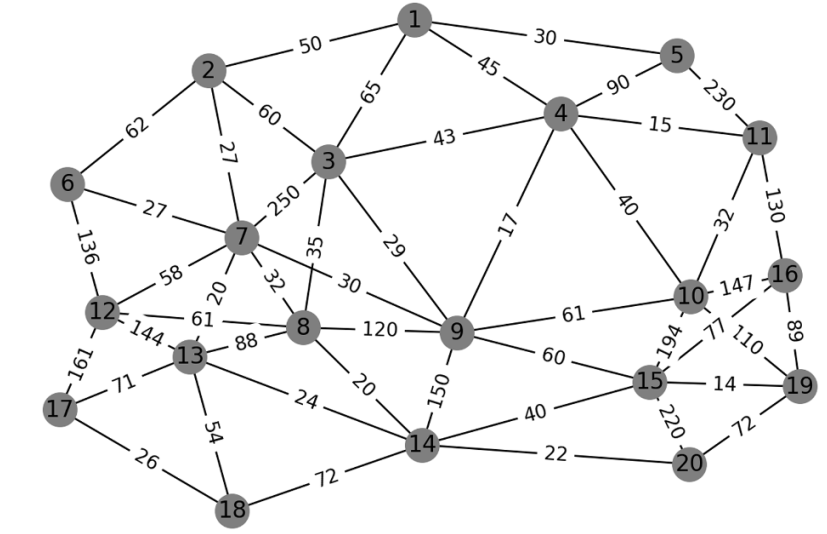
\includegraphics[width=6cm]{tsp_fig}
\caption{\label{img:tsp_fig}Exemplo de grafo para TSP.} 
\end{figure}

Algoritmos genéticos são meta heurística adaptativos que são classificados como um algoritmos de computação evolucionária, que usam técnicas inspiradas na evolução natural. O primeiro GA foi desenvolvido pela Holanda em 1975, para resolver alguns problemas de otimização, com base na genética biológica
e idéias evolucionárias \cite{ga}. A Fig. \ref{img:ga}  descreve um GA típico \cite{m-c}.

\begin{figure}[ht]
\centering
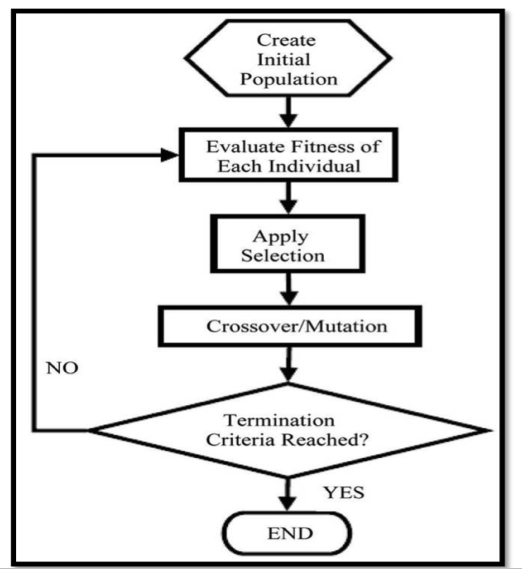
\includegraphics[width=6cm]{ga.png}
\caption{\label{img:ga}Fluxograma de um GA típico.} 
\end{figure}

O objeitvo deste trabalho é descrever e avaliar estudos relacionados às mudanças dinâmicas dos parâmetros de mutação e crossover, para otimizar um GA, para solucionar o problema de menro percurso entre duas cidades no TSP.

Nas seções materiais e métodos serão demonstrados como foram realizados os trabalhos, nos resultados e discussões os dados de resultados serão analisados e por fim haverá as conclusões. 


\section{Materiais e Métodos para o artigo \cite{fga}}
\label{sec:materials}
Nesta seção será demonstrada a metologia utilizada, materiais e paramêtros utilizados no FGA \cite{fga}, além demonstrar o pseudo-código.

Para simular o método proposto, utilizou-se o software Matlab
versão 2015a, com um computador com cpu intel i7, 2.3Ghz e
16 GB de RAM. 

Para o TSP, foram utilizados problemas com 10, 30 e 50 cidades, gerados pelos autores, para comparar FGA e GA. Além disso, foram utilizadas bases de dados públicas, chamadas de Eil51, Eil76, KroA100, com 51, 76 e 100 cidades, respectivamente, para comparar FGA, GA e outras metaheurísticas.

O pseudocódigo \ref{alg:1} demonstra a ideia de funcionamento do algoritmo original. No artigo não foi descrito como foi adquirida a população inicial, como funciona a seleção e função fitness.

\begin{algorithm}[ht]
\label{alg:1}
 \KwData{O número de gerações é 100, a população inicial, o método de seleção e a função fitness não são detalhados no trabalho.}
\Begin{
 Na primeira etapa, as melhores respostas da população de entrada são colocadas em uma variável chamda $fitness$ (vetor cuja cada posição tem um indivíduo, o qual represena um percurso completo).
    
Na segunda etapa, o desvio padrão da variável de $fitness$ é calculado e o resultado é inserido na variável $std$.
    
Na terceira etapa, a média e o máximo da variável $fitness$ são coletadas e inseridas nas variáveis $med$  e $max$, respectivamente.
    
Então, o número de cromossomos com maior $fitness$ que
    $med - std$ são contados e considerados como comossomos ruins ($G_W$, do inglês).
    
E  o número de cromossomos com menor $fitness$ do que $med + std$  são contados e considerados como genomas bons ($G_B$, do inglês).
    
    Nesta etapa, $G_B$ e genomas ruins ($G_W$, do inglês) são divididos pelo total de cromossomos para serem normalizado e se tornar $G_B_n$ e $G_W_n$.
    
    Então valores $G_W_n$ e $G_B_n$ são dados ao sistema fuzzy e este sistema produz $dPc$ e $dPm$, que são variáveis que alteram as taxas de crossover e mutação, respectivamente.
}
\caption{Proposta do FGA}
\label{alg:alg}
\end{algorithm}


Na equação \ref{eq:G_B_n} foi realizada uma normalização do total de genomas bons ($G_B$), dividido pelo o total de genomas, soluções ou arestas do TSP ($size(fitness)$), resultando em $G_B_n$. Na equação \ref{eq:G_W_n} acontece algo semelhante à equação \ref{eq:G_B_n}, porém com genomas ruins ($G_W$), cuja saída é $G_W_n$.
\begin{equation}
\label{eq:G_B_n}
    G_B_n = \frac{G_B}{size(fitness)}
\end{equation} 

\begin{equation}
\label{eq:G_W_n}
    G_W_n = \frac{G_W}{size(fitness)}
\end{equation} 

A Fig. \ref{img:fuzzy_fig1} demonstra a estratégica deste trabalho. Resumidamente, quando o número de cromossomos bons é alto e o número de cromossomos ruins é baixo, então a mutação e o crossover devem acontecer menos, para preservar as soluções (cromossomos) boas que existe em abundância. Porém, caso tanto os $G_B$ como $G_W$ sejam muitos, então a mutação deve acontecer menos e o crossover deve ocorrer com maior frequência, para tentar preservar um pouco da população boa e não perdê-las nas mutações. Conforme o crossover aumenta, melhores soluções serão alcançadas. 
\begin{figure}[ht]
\centering
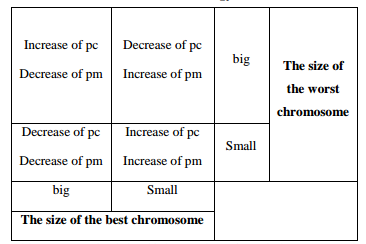
\includegraphics[width=6cm]{fuzzy_fig1.png}
\caption{\label{img:fuzzy_fig1}Tabela com estratégia da lógica fuzzy.} 
\end{figure}

A estratégia contida na tabela da Fig. \ref{img:fuzzy_fig1}, pode ser representada pela lógica fuzzy, como é demonstrado nas figuras Fig. \ref{img:fuzzy_fig2} e Fig. \ref{img:fuzzy_fig3} , onde $PB$ representa a problablidade de muitos e $PS$ a probabilidade de poucos genomas para $G_B_n$ ou  $G_W_n$, sendo estas duas última variáveis de entradas. Já as saídas podem ser do tipo $NP$ e $PB$. Na Fig. \ref{img:fuzzy_fig2}, uma resultante do tipo $NB$, resultará como consequência em $d_P_c$ negativo, por meio da função de pertinência encontrada na Fig \ref{img:fuzzy_pertinencia},  em contra partida $PB$ como resultado, gerará $d_P_c$ positivo, reduzindo e aumentando a taxa de mutação ($P_m$), respectvamente. O conceito de porta lógica $XNOR$ se aplica neste caso, ou seja, somente quando $G_B_n$ e $G_W_n$ forem diferentes, terá $PB$ na saída. Desta forma desestimula o crossover quando é desvantajoso, por exemplo, quando $G_B_n$ é pequeno e $G_W_n$ é grande, havendo menos herança de genes ruins.

\begin{figure}[ht]
\centering
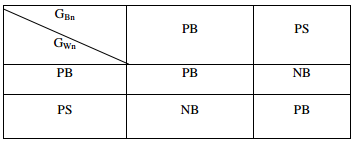
\includegraphics[width=6cm]{fuzzy_fig2.png}
\caption{\label{img:fuzzy_fig2}Tabela com lógica fuzzy para alterar o valor de $d_P_c$} 
\end{figure}

Já na figura \ref{img:fuzzy_fig3}, a saída depende apenas dos genomas bons, ou seja, quando  $G_B_n$ for grande, haverá $NB$ na saída para desestimular mutações e preservar boas soluções, do contrário, haverá $PB$  na saída para estimular mutações, reduzindo e aumentando $d_P_m$, respectivamente e, como consequência, a taxa de mutação ($P_m$). 
\begin{figure}[ht]
\centering
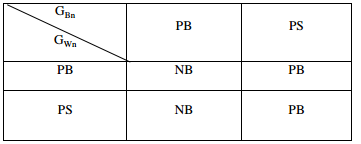
\includegraphics[width=6cm]{fuzzy_fig3.png}
\caption{\label{img:fuzzy_fig3}Tabela com lógica fuzzy para alterar o valor de $d_P_m$} 
\end{figure}

\begin{figure}[ht]
\centering
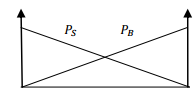
\includegraphics[width=6cm]{fuzzy_pertinencia.png}
\caption{\label{img:fuzzy_pertinencia} Função de pertinência} 
\end{figure}

Na equação \ref{eq:P_c} e \ref{eq:P_m} ocorre o processo conhecido como Defuzzytication, onde $dP_c$ e $dP_m$ agora se comportam como entradas. Na primeira equação, a nova taxa de crossover ($P_c$) depende da soma da taxa de crossover anterior ($P_c-1$) com o produto de uma constante ($k_c$), que é encontrada por tentativa e erro, com a variável que altera o crossover ($dP_c$), a qual pode ser postivida ou negativa de acordo com o processo fuzzy. A equação \ref{eq:P_m} segue a mesma ideia, porém para a taxa de mutação.

\begin{equation}
\label{eq:P_c}
    P_c(i) = P_c(i-1) + k_c dP_c(i) 
\end{equation}

\begin{equation}
\label{eq:P_m}
    P_m(i) = P_m(i-1) + k_m dP_m(i) 
\end{equation}
%até aqui

\section{Resultados e Discussão para o artigo \cite{fga}}
\label{sec:results}
Nesta seção serão apresentados os resultados comparando os percursos percorridos entre dois pontos em um grafo. Para testes com 10, 30 e 50 cidades, para o TSP, o FGA teve um menor percurso que GA, porém com maior tempo, como demonstrado na tabela da Fig. \ref{img:fuzzy_fig5}. Na figura \ref{img:fuzzy_fig6}, FGA demonstra melhor resultado para todos as bases de dados, onde o programa foi executado 20 vezes e utilizado os melhores resultados de cada um na tabela.

\begin{figure}[ht]
\centering
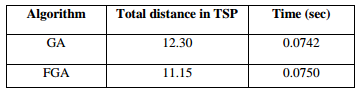
\includegraphics[width=6cm]{fuzzy_fig5.png}
\caption{\label{img:fuzzy_fig5} Resultados para 50 cidades} 
\end{figure}

\begin{figure}[ht]
\centering
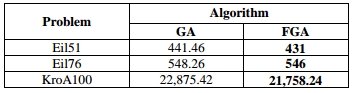
\includegraphics[width=6cm]{fuzzy_fig6.png}
\caption{\label{img:fuzzy_fig6} Resultados para as três bases de dados públicas diferentes} 
\end{figure}

Por fim, houve uma comparação entre FGA com outras metaheurística, onde FGA demonstrou bons resultados para bases de dados com menos números de cidades, conforme Fig. \ref{img:fuzzy_fig7}.
\begin{figure}[ht]
\centering
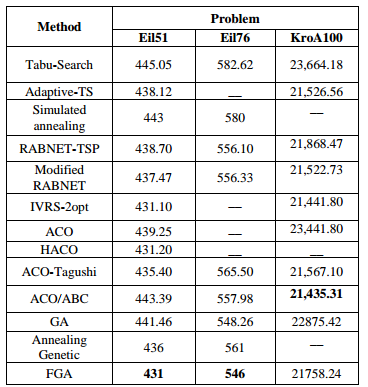
\includegraphics[width=6cm]{fuzzy_fig7.png}
\caption{\label{img:fuzzy_fig7} Resultados comparativos entre FGA e outras metaheurísticas} 
\end{figure}

Nos testes apenas entre FGA e GA, o primeiro apresentou uma pequena redução do percurso total para o problema do TSP, porém gastou mais tempo quando comparado com o GA tradicional. Além isso, o trabalho apresentou melhores soluções quando se compara FGA com algumas outras metaheurírsticas para o número de cidades 51 e 76, em contra-partida FGA é um dos piores para 100 cidades. Devido à pequena redução do percurso e aumentao do tempo do FGA quando comparado ao GA, ainda somando a limitações no número e tipos de testes, é difícil definir o FGA com maior eficácia em problemas mais abrangentes. Seriam necessários mais testes em maior amplitude de problemas.

\section{Materiais e Métodos para o artigo \cite{m-c}}
\label{sec:materials}
Nesta seção será desmonstrada como foi realizado os experimentos para o artigo \cite{m-c}.

Para todos os testes, os parametros do GA foram: a população inicial foi gerada aleatoriamente; método de seleção por roleta; função fitness depende do problema; mutação seleciona dois genes aleatoriamente entre duas posições de um indivíduo; o crossover escolhe pontos aleatórios dos pais; número de gerações com valor fixo de 1600; os indivíduos são representados por vetores contendo soluções (genomas ou arestas) em cada posição, trilhando o percurso da cidade de origem até a cidade de destino. 
Os testes foram realiazados com população de 25, 50, 100, 200, 300 e 400 indivíduos, com 1600 gerações, com os problemas TSP(rat783), TSP(pr144), TSP(eil51),TSP(berlin52), TSP(pr76), TSP(KroA100), TSP(att48), TSP(u159), TSP(a280) e TSP(ch130). Houveram um total 54 testes, variando-se o tamanho da população e número de cidades. 

A proposta deste trabalho é demonstrar duas ténicas: DHM/ILC, cujo a mutação começa com valor alto e vai reduzindo ao passar das gerações e a taxa de crossover começa baixa e vai aumentando com o passar das gerações,  conforme demonstrado a Fig. \ref{img:m-c_dhm-ilc} ; e ILM/DHC, que é o contrário, onde a taxa de mutação começa baixa e vai se incrementado com o passar das épocas, e a taxa de crossover começa alta e vai reduzindo, conforme a Fig. \ref{img:m-c_ilm-dhc}. Além da comparação entre as duas téncias mencionados, foram comparadas mais duas téncias com taxas de mutação e crossover estáticas: a primeira técnica com a proporção de 30\% de taxa de mutação e 90\% de taxa de crossover, chamada de  0.03MR0.9CR; a outra técnica, conhecida como FFMCR, utilizada  50\% para ambas as taxas.

Para a técnica de ILM/DHC, cálculo da taxa de mutação para cada época é dado pela equação \ref{eq:MR1} , onde $Gn$ representa o número total de gerações, $LG$ é o número da geração atual e MR é a taxa de mutação. Na equação \ref{eq:M1}, $M$ é a parcela da população que soferá a mutação, multiplicando $MR$ por $popsize$, que é o tamanho total da população.
$CR$ é a taxa de crossover e $C$ é a parcela da população que sofrerá cruzamento, conforme as equações \ref{eq:CR1} e \ref{eq:C1}. $CR$ funciona como complemento de $MR$, ou seja, são inversamente proporcional.

\begin{equation}
\label{eq:MR1}
    MR = \frac{LG}{Gn}
\end{equation}

\begin{equation}
\label{eq:M1}
    M = MR * popsize    
\end{equation}

\begin{equation}
\label{eq:CR1}
    CR = 1 - \frac{LG}{Gn}
\end{equation}

\begin{equation}
\label{eq:C1}
    C = CR * popsize    
\end{equation}

No DHM/ILC, para cálcula a taxa de mutação, utiliza-se as equações \ref{eq:MR2}, \ref{eq:M2}, e para cálcular a taxa de crossover, usa-se as equações \ref{eq:CR2}, \ref{eq:C2}, seguindo uma lógica inversa à ILM/DHC.
\begin{equation}
\label{eq:MR2}
    MR = 1 - \frac{LG}{Gn}
\end{equation}

\begin{equation}
\label{eq:M2}
    M = MR * popsize    
\end{equation}

\begin{equation}
\label{eq:CR2}
    CR = \frac{LG}{Gn}
\end{equation}

\begin{equation}
\label{eq:C2}
    C = CR * popsize    
\end{equation}

\begin{figure}[ht]
\centering
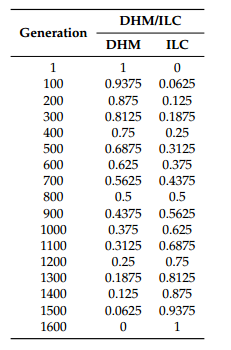
\includegraphics[width=6cm]{m-c_dhm-ilc.png}
\caption{\label{img:m-c_dhm-ilc} Taxas de cruzamento e mutação durante a execução de GA usando diminuição de mutação alta (DHM) e incremento de crossover baixo (ILC) } 
\end{figure}

\begin{figure}[ht]
\centering
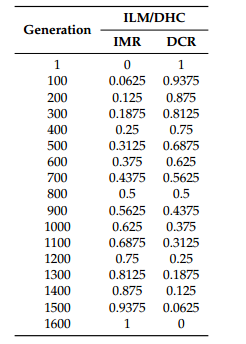
\includegraphics[width=6cm]{m-c_ilm-dhc.png}
\caption{\label{img:m-c_ilm-dhc} Taxas de cruzamento e mutação durante a execução de GA usando incremento de mutação baixa (ILM) e redução de crossover alto (DHC) } 
\end{figure}



\section{Resultados e Discussão para o artigo \cite{m-c}}
Nesta seção serão apresentados os resultados e discutidos para o aritgo \cite{m-c}. Houveram muitos testes com várias bases de dados, que podem ser verificados no artigo original, porém aqui será demonstrada apenas uma parcela dos resultados. 

O gráfico da Fig. \ref{img:m-c_barra_size25}, ILM/DHC converge para uma melhor solução, quando comparado a outras técnicas, para população de 25 indivíduos, após 1600 gerações, para o problema TSP/kro100 com 100 vértices. O gráfico boxplot da Fig. \ref{img:m-c_boxplot_size25} demonstra que a téncnica ILM/DHC tem melhores soluções na maior parte das vezes, com menores variâncias para vários problemas de TSP. 

\begin{figure}[ht]
\centering
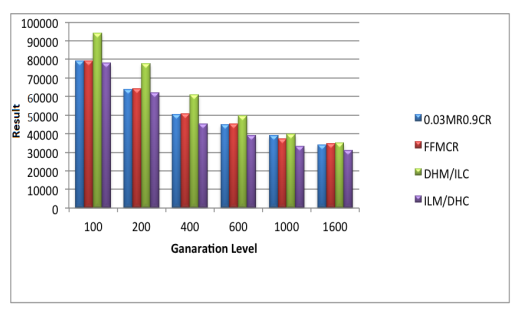
\includegraphics[width=6cm]{m-c_barra_size25.png}
\caption{\label{img:m-c_barra_size25} Gráfico barra para população de 25 e o problema TSP/kro100 } 
\end{figure}

\begin{figure}[ht]
\centering
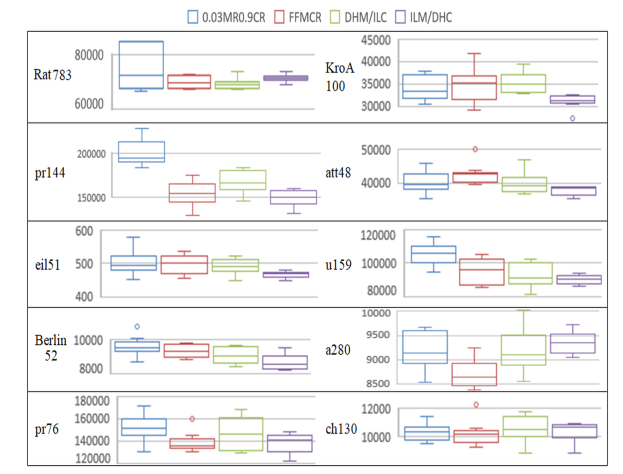
\includegraphics[width=6cm]{m-c_boxplot_size25.png}
\caption{\label{img:m-c_boxplot_size25} Gráfico boxplot para população de 25 e vários problemas do TSP} 
\end{figure}

No gráfico da Fig. \ref{img:m-c_barra_size400}, DHM/ILC converge para uma melhor solução comparado a outras técnicas, para população de 400 indivíduos, 1600 gerações e o problema TSP/kro100. O gráfico boxplot da Fig. \ref{img:m-c_boxplot_size400} demonstra que a técnica DHM/ILC resulta em melhores soluções e menores variâncias na maior parte dos problemas TSP. 

\begin{figure}[ht]
\centering
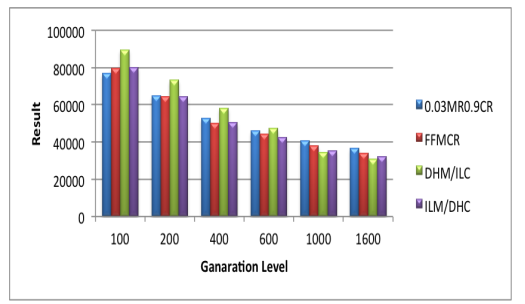
\includegraphics[width=6cm]{m-c_barra_size400.png}
\caption{\label{img:m-c_barra_size400} Gráfico barra para população de 400 e o problema TSP/kro100 } 
\end{figure}

\begin{figure}[ht]
\centering
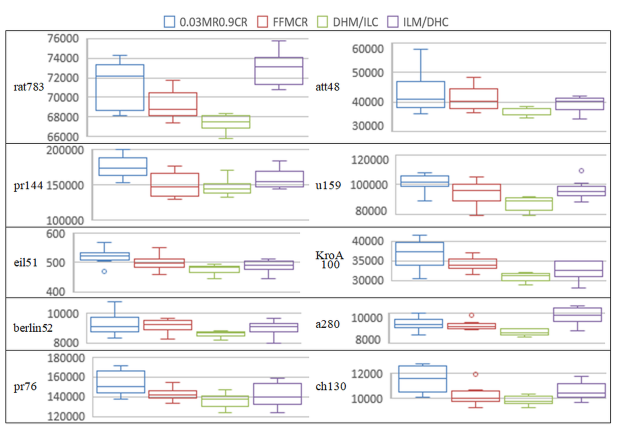
\includegraphics[width=6cm]{m-c_boxplot_size400.png}
\caption{\label{img:m-c_boxplot_size400} Gráfico boxplot para população de 400 e vários problemas do TSP} 
\end{figure}

Para o menor número de cidades, a técnica ILM/DHC apresenta melhores soluções, porém a medida que se aumenta o números de vértices (cidades), a técnica DHM/ILC demonstra melhores resultados. As técnicas de mutação e crossover estáticos, 0.03MR0.9CR e FFMCR, demonstram piores soluções e maiores varianças na grande maioria dos testes. 

Os resultados do estudo \cite{m-c} demonstraram maior solidez em relação ao estudo \cite{fga} devido a quantidade de testes e análises estatíticas. Mesmo assim o trabalho ainda tem limitações de amostras e não deve ser abrangente a todos os problemas TSP.

\section{Conclusão}

\label{sec:conclusion}

%antigo
Este trabalho apresentou dois estudos a respeito da mutação e crossover dinâmico em um GA. 
Em relação ao primeiro estudo \cite{fga}, como ponto positivo, houve ligeira redução do percurso total do FGA em relação ao GA em todos casos testados e melhoras em relação a outras metaheurísticas para 51 e 76 cidades. Alguns pontos negativos deste artigo é que ele não apresenta alguns dados, como a população inicial, função fitness, método de seleção, além de alguns outros problemas como ter que definir $k_c$ e $k_m$ por tentativa de erro, e não definir quantitativamente o que seria uma população grande e pequena de genomas. Há ainda o problema de ter que entender alguns dados e variáveis por dedução.

Em relação ao segundo estudo \cite{m-c}, ele foi mais claro quando à dados de parâmetros, técnicas e ainda realizou uma grande quantidade de testes variados. Um problema deste estudo é que as soluções das técnicas podem não ser tão expressivas, quando comparadas a outra técnicas, dependendo da situação onde for utilizada. Ainda faltou a medição de tempo de execução das metaheurísticas, pois um tempo muito maior para o FGA pode não justificar um pouco de melhora na sua solução. Por último não foi descrito em que condições computacionais foram realizados os testes, pois ambientes e situações diferentes podem gerar dados enviesados.

Os estudos parecem promissores, porém se deve considerá-los apenas para os casos testados e as possíveis falhas. Ambos podem servir como base para novos trabalhos.

\newpage 
\bibliographystyle{unsrt}
\bibliography{icdp2009}

\end{document}